


\tikzset{every picture/.style={line width=0.75pt}} %set default line width to 0.75pt        

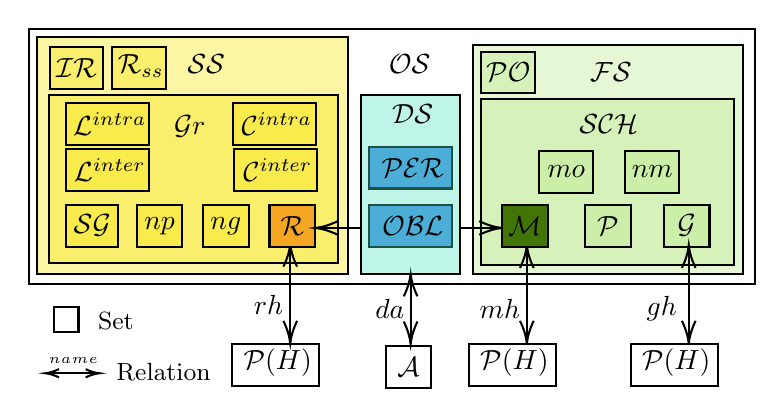
\begin{tikzpicture}[x=0.75pt,y=0.75pt,yscale=-1,xscale=1]
%uncomment if require: \path (0,1800); %set diagram left start at 0, and has height of 1800

%Shape: Rectangle [id:dp9341453924522656] 
\draw  [fill={rgb, 255:red, 255; green, 255; blue, 255 }  ,fill opacity=1 ] (160,44) -- (510,44) -- (510,167) -- (160,167) -- cycle ;
%Shape: Rectangle [id:dp4628140741854456] 
\draw  [fill={rgb, 255:red, 184; green, 233; blue, 134 }  ,fill opacity=0.34 ] (374,52) -- (504,52) -- (504,162) -- (374,162) -- cycle ;
%Shape: Rectangle [id:dp6461749357206974] 
\draw  [fill={rgb, 255:red, 184; green, 233; blue, 134 }  ,fill opacity=0.34 ] (378,78) -- (500,78) -- (500,158) -- (378,158) -- cycle ;
%Shape: Rectangle [id:dp47018118728898073] 
\draw  [fill={rgb, 255:red, 248; green, 231; blue, 28 }  ,fill opacity=0.4 ] (164,48) -- (314,48) -- (314,162) -- (164,162) -- cycle ;
%Straight Lines [id:da37904402438854] 
\draw    (400,150.31) -- (400,193.69) ;
\draw [shift={(400,195.69)}, rotate = 270] [color={rgb, 255:red, 0; green, 0; blue, 0 }  ][line width=0.75]    (10.93,-3.29) .. controls (6.95,-1.4) and (3.31,-0.3) .. (0,0) .. controls (3.31,0.3) and (6.95,1.4) .. (10.93,3.29)   ;
\draw [shift={(400,148.31)}, rotate = 90] [color={rgb, 255:red, 0; green, 0; blue, 0 }  ][line width=0.75]    (10.93,-3.29) .. controls (6.95,-1.4) and (3.31,-0.3) .. (0,0) .. controls (3.31,0.3) and (6.95,1.4) .. (10.93,3.29)   ;
%Straight Lines [id:da30557994145553513] 
\draw    (368,140) -- (386,140) ;
\draw [shift={(388,140)}, rotate = 180] [color={rgb, 255:red, 0; green, 0; blue, 0 }  ][line width=0.75]    (10.93,-3.29) .. controls (6.95,-1.4) and (3.31,-0.3) .. (0,0) .. controls (3.31,0.3) and (6.95,1.4) .. (10.93,3.29)   ;
%Shape: Rectangle [id:dp15689957472567295] 
\draw  [fill={rgb, 255:red, 248; green, 231; blue, 28 }  ,fill opacity=0.4 ] (169.56,76) -- (309.06,76) -- (309.06,157) -- (169.56,157) -- cycle ;
%Shape: Rectangle [id:dp6202366628126772] 
\draw  [fill={rgb, 255:red, 255; green, 255; blue, 255 }  ,fill opacity=1 ] (372,196) -- (414,196) -- (414,216) -- (372,216) -- cycle ;

%Shape: Rectangle [id:dp20067598884831228] 
\draw  [fill={rgb, 255:red, 248; green, 231; blue, 28 }  ,fill opacity=0.4 ] (212.06,129) -- (234.06,129) -- (234.06,149) -- (212.06,149) -- cycle ;

%Shape: Rectangle [id:dp5970765798398485] 
\draw  [fill={rgb, 255:red, 248; green, 231; blue, 28 }  ,fill opacity=0.4 ] (178.06,129) -- (203.06,129) -- (203.06,149) -- (178.06,149) -- cycle ;
%Shape: Rectangle [id:dp92237875722883] 
\draw  [fill={rgb, 255:red, 248; green, 231; blue, 28 }  ,fill opacity=0.4 ] (178.06,102) -- (218.06,102) -- (218.06,122) -- (178.06,122) -- cycle ;

%Shape: Rectangle [id:dp6591761395302378] 
\draw  [fill={rgb, 255:red, 248; green, 231; blue, 28 }  ,fill opacity=0.4 ] (178.06,80) -- (218.06,80) -- (218.06,100) -- (178.06,100) -- cycle ;

%Shape: Rectangle [id:dp11794703752595392] 
\draw  [fill={rgb, 255:red, 248; green, 231; blue, 28 }  ,fill opacity=0.4 ] (258.5,80) -- (298.5,80) -- (298.5,100) -- (258.5,100) -- cycle ;

%Shape: Rectangle [id:dp6557958558103134] 
\draw  [fill={rgb, 255:red, 248; green, 231; blue, 28 }  ,fill opacity=0.4 ] (259,102) -- (299,102) -- (299,122) -- (259,122) -- cycle ;

%Shape: Rectangle [id:dp8284992701408749] 
\draw  [fill={rgb, 255:red, 65; green, 117; blue, 5 }  ,fill opacity=1 ] (388,129) -- (410,129) -- (410,149) -- (388,149) -- cycle ;

%Shape: Rectangle [id:dp7066110016250453] 
\draw  [fill={rgb, 255:red, 248; green, 231; blue, 28 }  ,fill opacity=0.4 ] (244,129) -- (266,129) -- (266,149) -- (244,149) -- cycle ;

%Shape: Rectangle [id:dp4021333114319714] 
\draw  [fill={rgb, 255:red, 248; green, 231; blue, 28 }  ,fill opacity=0.4 ] (170.31,53) -- (195.69,53) -- (195.69,73) -- (170.31,73) -- cycle ;

%Shape: Rectangle [id:dp8476756388266236] 
\draw  [fill={rgb, 255:red, 248; green, 231; blue, 28 }  ,fill opacity=0.4 ] (200,53) -- (226,53) -- (226,73) -- (200,73) -- cycle ;

%Shape: Rectangle [id:dp07470576340681823] 
\draw  [fill={rgb, 255:red, 74; green, 144; blue, 226 }  ,fill opacity=1 ] (324,101) -- (364,101) -- (364,121) -- (324,121) -- cycle ;

%Shape: Rectangle [id:dp31407652093057714] 
\draw  [fill={rgb, 255:red, 74; green, 144; blue, 226 }  ,fill opacity=1 ] (324,129) -- (364,129) -- (364,149) -- (324,149) -- cycle ;

%Shape: Rectangle [id:dp053729126169398844] 
\draw  [fill={rgb, 255:red, 184; green, 233; blue, 134 }  ,fill opacity=0.34 ] (378,55) -- (404,55) -- (404,75) -- (378,75) -- cycle ;

%Shape: Rectangle [id:dp7720103442630182] 
\draw  [fill={rgb, 255:red, 184; green, 233; blue, 134 }  ,fill opacity=0.34 ] (405.94,103) -- (431.94,103) -- (431.94,123) -- (405.94,123) -- cycle ;

%Shape: Rectangle [id:dp3183552657000306] 
\draw  [fill={rgb, 255:red, 184; green, 233; blue, 134 }  ,fill opacity=0.34 ] (447.44,103) -- (473.44,103) -- (473.44,123) -- (447.44,123) -- cycle ;

%Shape: Rectangle [id:dp10802424702469593] 
\draw  [fill={rgb, 255:red, 184; green, 233; blue, 134 }  ,fill opacity=0.34 ] (466,129) -- (488,129) -- (488,149) -- (466,149) -- cycle ;

%Shape: Rectangle [id:dp16589412198505937] 
\draw  [fill={rgb, 255:red, 184; green, 233; blue, 134 }  ,fill opacity=0.34 ] (428,129) -- (450,129) -- (450,149) -- (428,149) -- cycle ;

%Shape: Rectangle [id:dp1270989692188249] 
\draw  [fill={rgb, 255:red, 255; green, 255; blue, 255 }  ,fill opacity=1 ] (258,196) -- (300,196) -- (300,216) -- (258,216) -- cycle ;

%Straight Lines [id:da40017392935840324] 
\draw    (286,149.69) -- (286,193.69) ;
\draw [shift={(286,195.69)}, rotate = 270] [color={rgb, 255:red, 0; green, 0; blue, 0 }  ][line width=0.75]    (10.93,-3.29) .. controls (6.95,-1.4) and (3.31,-0.3) .. (0,0) .. controls (3.31,0.3) and (6.95,1.4) .. (10.93,3.29)   ;
\draw [shift={(286,147.69)}, rotate = 90] [color={rgb, 255:red, 0; green, 0; blue, 0 }  ][line width=0.75]    (10.93,-3.29) .. controls (6.95,-1.4) and (3.31,-0.3) .. (0,0) .. controls (3.31,0.3) and (6.95,1.4) .. (10.93,3.29)   ;
%Shape: Rectangle [id:dp21027747628033966] 
\draw  [fill={rgb, 255:red, 245; green, 166; blue, 35 }  ,fill opacity=1 ] (276,129) -- (298,129) -- (298,149) -- (276,149) -- cycle ;

%Shape: Rectangle [id:dp5582162899072272] 
\draw  [fill={rgb, 255:red, 255; green, 255; blue, 255 }  ,fill opacity=1 ] (172,178) -- (184,178) -- (184,190) -- (172,190) -- cycle ;
%Straight Lines [id:da3472969066473863] 
\draw    (170,210) -- (192,210) ;
\draw [shift={(194,210)}, rotate = 180] [color={rgb, 255:red, 0; green, 0; blue, 0 }  ][line width=0.75]    (6.56,-1.97) .. controls (4.17,-0.84) and (1.99,-0.18) .. (0,0) .. controls (1.99,0.18) and (4.17,0.84) .. (6.56,1.97)   ;
\draw [shift={(168,210)}, rotate = 0] [color={rgb, 255:red, 0; green, 0; blue, 0 }  ][line width=0.75]    (6.56,-1.97) .. controls (4.17,-0.84) and (1.99,-0.18) .. (0,0) .. controls (1.99,0.18) and (4.17,0.84) .. (6.56,1.97)   ;
%Shape: Rectangle [id:dp07012270906311535] 
\draw  [fill={rgb, 255:red, 255; green, 255; blue, 255 }  ,fill opacity=1 ] (332,197) -- (354,197) -- (354,217) -- (332,217) -- cycle ;

%Straight Lines [id:da7534392810513293] 
\draw    (344,164) -- (344,194) ;
\draw [shift={(344,196)}, rotate = 270] [color={rgb, 255:red, 0; green, 0; blue, 0 }  ][line width=0.75]    (10.93,-3.29) .. controls (6.95,-1.4) and (3.31,-0.3) .. (0,0) .. controls (3.31,0.3) and (6.95,1.4) .. (10.93,3.29)   ;
\draw [shift={(344,162)}, rotate = 90] [color={rgb, 255:red, 0; green, 0; blue, 0 }  ][line width=0.75]    (10.93,-3.29) .. controls (6.95,-1.4) and (3.31,-0.3) .. (0,0) .. controls (3.31,0.3) and (6.95,1.4) .. (10.93,3.29)   ;
%Straight Lines [id:da4125176624573814] 
\draw    (320,140) -- (300,140) ;
\draw [shift={(298,140)}, rotate = 360] [color={rgb, 255:red, 0; green, 0; blue, 0 }  ][line width=0.75]    (10.93,-3.29) .. controls (6.95,-1.4) and (3.31,-0.3) .. (0,0) .. controls (3.31,0.3) and (6.95,1.4) .. (10.93,3.29)   ;
%Shape: Rectangle [id:dp005426842763594397] 
\draw  [fill={rgb, 255:red, 80; green, 227; blue, 194 }  ,fill opacity=0.36 ] (320,76) -- (368,76) -- (368,162) -- (320,162) -- cycle ;
%Straight Lines [id:da9128713017721406] 
\draw    (478,150.31) -- (478,193.69) ;
\draw [shift={(478,195.69)}, rotate = 270] [color={rgb, 255:red, 0; green, 0; blue, 0 }  ][line width=0.75]    (10.93,-3.29) .. controls (6.95,-1.4) and (3.31,-0.3) .. (0,0) .. controls (3.31,0.3) and (6.95,1.4) .. (10.93,3.29)   ;
\draw [shift={(478,148.31)}, rotate = 90] [color={rgb, 255:red, 0; green, 0; blue, 0 }  ][line width=0.75]    (10.93,-3.29) .. controls (6.95,-1.4) and (3.31,-0.3) .. (0,0) .. controls (3.31,0.3) and (6.95,1.4) .. (10.93,3.29)   ;
%Shape: Rectangle [id:dp7604827971406838] 
\draw  [fill={rgb, 255:red, 255; green, 255; blue, 255 }  ,fill opacity=1 ] (450,196) -- (492,196) -- (492,216) -- (450,216) -- cycle ;



% Text Node
\draw (465,179) node   [align=left] {$gh$};
% Text Node
\draw (181.5,204) node  [font=\tiny] [align=left] {$name$};
% Text Node
\draw (334,179) node   [align=left] {$da$};
% Text Node
\draw (222,207) node  [font=\footnotesize] [align=left] {\begin{minipage}[lt]{29.67pt}\setlength\topsep{0pt}
\begin{center}
{\small Relation}
\end{center}

\end{minipage}};
% Text Node
\draw (202,185) node  [font=\footnotesize] [align=left] {\begin{minipage}[lt]{13.75pt}\setlength\topsep{0pt}
\begin{center}
{\small Set}
\end{center}

\end{minipage}};
% Text Node
\draw (343.5,61) node   [align=left] {$\mathcal{OS}$};
% Text Node
\draw (190.56,139) node   [align=left] {$\mathcal{SG}$};
% Text Node
\draw (345,85) node   [align=left] {$\mathcal{DS}$};
% Text Node
\draw (245.5,61) node   [align=left] {$\mathcal{SS}$};
% Text Node
\draw (387,179) node   [align=left] {$mh$};
% Text Node
\draw (275.5,177) node   [align=left] {$rh$};
% Text Node
\draw (237.56,91) node   [align=left] {$\mathcal{G}r$};
% Text Node
\draw (440.5,65) node   [align=left] {$\mathcal{FS}$};
% Text Node
\draw (439.44,90) node   [align=left] {$\mathcal{SCH}$};
% Text Node
\draw (472,205) node   [align=left] {$\mathcal{P}(H)$};
% Text Node
\draw (343,207) node   [align=left] {$\mathcal{A}$};
% Text Node
\draw (287,139) node   [align=left] {$\mathcal{R}$};
% Text Node
\draw (280,205) node   [align=left] {$\mathcal{P}(H)$};
% Text Node
\draw (439,139) node   [align=left] {$\mathcal{P}$};
% Text Node
\draw (477,139) node   [align=left] {$\mathcal{G}$};
% Text Node
\draw (460.44,113) node   [align=left] {$nm$};
% Text Node
\draw (418.94,113) node   [align=left] {$mo$};
% Text Node
\draw (391,65) node   [align=left] {$\mathcal{PO}$};
% Text Node
\draw (345,139) node   [align=left] {$\mathcal{OBL}$};
% Text Node
\draw (345,111) node   [align=left] {$\mathcal{PER}$};
% Text Node
\draw (214,62) node   [align=left] {$\mathcal{R}_{ss}$};
% Text Node
\draw (183,63) node   [align=left] {$\mathcal{IR}$};
% Text Node
\draw (255,139) node   [align=left] {$\mathnormal{ng}$};
% Text Node
\draw (399,139) node   [align=left] {$\mathcal{M}$};
% Text Node
\draw (280,112) node   [align=left] {$\mathcal{C}^{inter}$};
% Text Node
\draw (279.5,90) node   [align=left] {$\mathcal{C}^{intra}$};
% Text Node
\draw (199.06,90) node   [align=left] {$\mathcal{L}^{intra}$};
% Text Node
\draw (199.06,112) node   [align=left] {$\mathcal{L}^{inter}$};
% Text Node
\draw (223.06,139) node   [align=left] {$np$};
% Text Node
\draw (394,205) node   [align=left] {$\mathcal{P}(H)$};


\end{tikzpicture}